\documentclass[11pt, letterpaper]{article}

\usepackage[margin=1in]{geometry}
\usepackage[T1]{fontenc}
\usepackage[utf8]{inputenc}
\usepackage{enumitem}
\usepackage{xcolor}
\usepackage{parskip}
\usepackage{booktabs}
\usepackage{tabularx}
\usepackage{tikz}
\usetikzlibrary{positioning, arrows.meta}
\usepackage{amsmath}

% Clean sans-serif font
\usepackage{helvet}
\renewcommand{\familydefault}{\sfdefault}

% Accent color
\definecolor{accent}{RGB}{51, 65, 85}

\begin{document}

\begin{center}
{\Large \textbf{The Mythical Man-Month}}\\[0.5em]
{\color{accent}\large Why Adding People Makes Projects Later}\\[0.3em]
{\small Based on Fred Brooks (1975, 1995) | \today}
\end{center}

\vspace{1.5em}

\section*{Introduction}

In 1975, Fred Brooks published \textit{The Mythical Man-Month}, drawing on his experience managing the development of IBM's OS/360---one of the largest and most complex software projects of its era. The book's central insight, now known as Brooks's Law, challenged the intuitive assumption that adding people to a project accelerates delivery. Nearly fifty years later, Brooks's observations remain the most influential framework for understanding why large software projects fail and what managers can do about it.

This paper summarizes the core concepts from \textit{The Mythical Man-Month} and explains why they matter for anyone managing complex technical projects.

\vspace{1em}

\section*{Brooks's Law}

\begin{center}
\textit{``Adding manpower to a late software project makes it later.''}
\end{center}

\vspace{0.5em}

This counterintuitive principle is the book's most famous contribution. Brooks observed that when a project falls behind schedule, the instinctive management response---adding more people---often makes the problem worse, not better.

\textbf{Why adding people slows projects down:}

\begin{enumerate}
    \item \textbf{Communication Overhead Scales Quadratically}
    
    If a team has $n$ people, the number of communication channels between them is:
    \[
    \frac{n(n-1)}{2}
    \]
    
    A 4-person team has 6 communication channels. A 10-person team has 45. A 15-person team has 105. As the team grows, the time spent coordinating, meeting, and resolving misunderstandings grows faster than the productive capacity added.
    
    \begin{center}
    \begin{tabular}{rr}
    \toprule
    \textbf{Team Size} & \textbf{Communication Channels} \\
    \midrule
    4 & 6 \\
    8 & 28 \\
    12 & 66 \\
    15 & 105 \\
    20 & 190 \\
    \bottomrule
    \end{tabular}
    \end{center}
    
    \item \textbf{The Learning Curve Consumes Capacity}
    
    New team members are not productive on Day 1. They must learn the codebase, the architecture, the conventions, the tools, and the domain. During this ramp-up period, they consume the time of experienced team members who must teach them. The project loses capacity from both the learners (who are not yet contributing) and the teachers (who are diverted from productive work).
    
    \item \textbf{Task Partitioning Has Limits}
    
    Not all work can be parallelized. Brooks uses the analogy of pregnancy: nine women cannot have a baby in one month. Software projects contain sequential dependencies---work that cannot begin until prior work is complete. Adding people to parallelize the parallelizable portions does not accelerate the sequential portions, which often define the critical path.
    
    \item \textbf{Integration Complexity Increases}
    
    More people means more independently developed components that must be integrated. Integration is where assumptions collide, interfaces mismatch, and bugs emerge. The more components, the more integration work---and integration work scales worse than linearly.
\end{enumerate}

\textbf{The Implication:} When a project is late, adding people may accelerate certain tasks while simultaneously slowing the overall project. The net effect is often negative, especially if the new people lack domain knowledge and the existing team is already stretched thin.

\vspace{1em}

\section*{Conceptual Integrity}

\begin{center}
\textit{``Conceptual integrity is the most important consideration in system design.''}
\end{center}

\vspace{0.5em}

Brooks argues that a well-designed system should feel like it was designed by a single mind. The user interface should be consistent. The architecture should follow coherent principles. The naming conventions, error handling, and data structures should reflect a unified vision.

\textbf{Why conceptual integrity matters:}

\begin{itemize}
    \item Systems with conceptual integrity are easier to learn, use, and maintain.
    \item Inconsistent systems confuse users and create opportunities for errors.
    \item Maintenance programmers can predict how unfamiliar parts of the system work based on patterns they've learned elsewhere in the system.
\end{itemize}

\textbf{How to achieve conceptual integrity:}

Brooks recommends that a small number of people---ideally one person, the system architect---own the design vision. The architect defines the interfaces, conventions, and principles. The implementation team builds to those specifications. This separation ensures that the system reflects a coherent vision rather than a committee compromise.

\textbf{The tradeoff:} Concentrating design authority in few hands may feel undemocratic, and implementers may chafe at constraints they did not choose. But Brooks argues this is the price of coherence. A camel is a horse designed by committee.

\vspace{1em}

\section*{The Surgical Team}

To reconcile the need for small teams (for conceptual integrity and low communication overhead) with the reality that large systems require many person-years of effort, Brooks proposes the \textbf{surgical team} model.

\textbf{How it works:}

A small, highly skilled core team (the ``surgeons'') does the critical design and implementation work. They are supported by specialists who handle tooling, testing, documentation, and administrative tasks. The surgeons make decisions; the support team amplifies their productivity.

\begin{center}
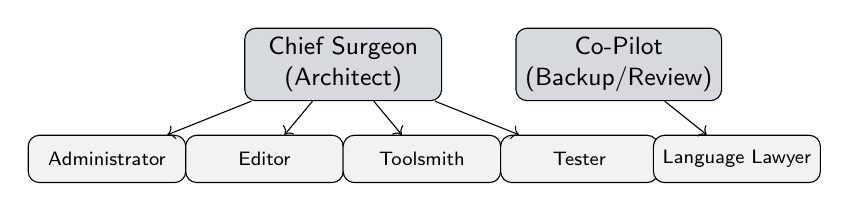
\begin{tikzpicture}[
    node distance=0.5cm,
    core/.style={draw, rounded corners=4pt, fill=accent!20, minimum width=2.5cm, minimum height=0.7cm, align=center, font=\small},
    support/.style={draw, rounded corners=4pt, fill=gray!10, minimum width=2cm, minimum height=0.6cm, align=center, font=\scriptsize}
]
    \node[core] (surgeon) at (0,0) {Chief Surgeon\\(Architect)};
    \node[core] (copilot) at (3.5,0) {Co-Pilot\\(Backup/Review)};
    
    \node[support] (admin) at (-3,-1.2) {Administrator};
    \node[support] (editor) at (-1,-1.2) {Editor};
    \node[support] (toolsmith) at (1,-1.2) {Toolsmith};
    \node[support] (tester) at (3,-1.2) {Tester};
    \node[support] (lang) at (5,-1.2) {Language Lawyer};
    
    \draw[->] (surgeon) -- (admin);
    \draw[->] (surgeon) -- (editor);
    \draw[->] (surgeon) -- (toolsmith);
    \draw[->] (surgeon) -- (tester);
    \draw[->] (copilot) -- (lang);
\end{tikzpicture}
\end{center}

\textbf{Why this works:}

\begin{itemize}
    \item The surgeons maintain conceptual integrity because they make all key decisions.
    \item Communication overhead is low because the core team is small.
    \item The support team handles work that would otherwise distract the surgeons.
    \item Total capacity is high because the support team multiplies the surgeons' output.
\end{itemize}

\textbf{The key insight:} Not all team members need to be interchangeable generalists. Specialization, with clear roles and interfaces, can scale a team without incurring the full communication penalty.

\vspace{1em}

\section*{No Silver Bullet}

In a 1986 essay later incorporated into the book, Brooks addressed the persistent hope that some new technology---structured programming, object-oriented design, AI, visual programming---would deliver a tenfold improvement in software productivity.

\begin{center}
\textit{``There is no single development, in either technology or management technique,\\which by itself promises even one order-of-magnitude improvement\\within a decade in productivity, in reliability, in simplicity.''}
\end{center}

\vspace{0.5em}

\textbf{Why there is no silver bullet:}

Brooks distinguishes between \textbf{essential complexity} (inherent in the problem being solved) and \textbf{accidental complexity} (introduced by inadequate tools or methods). Decades of progress have reduced accidental complexity---better languages, better tools, better frameworks. But essential complexity remains.

Software is hard because:
\begin{itemize}
    \item Requirements are complex, ambiguous, and changing.
    \item Systems must handle countless edge cases and failure modes.
    \item Software must integrate with other systems that have their own complexity.
    \item Users have diverse needs and mental models.
\end{itemize}

No tool eliminates this essential complexity. Tools can only reduce the friction of expressing solutions to complex problems---they cannot make the problems simpler.

\textbf{The implication:} Beware of vendors or methodologies promising dramatic productivity gains. Incremental improvements are realistic; revolutions are rare.

\vspace{1em}

\section*{The Second-System Effect}

\begin{center}
\textit{``The second system is the most dangerous system a man ever designs.''}
\end{center}

\vspace{0.5em}

Brooks observed a pattern: an architect's first system is often lean and focused, built under constraints that force discipline. Emboldened by success, the architect approaches the second system with ambition---all the features deferred from the first, all the ideas accumulated since. The result is often bloated, over-engineered, and late.

\textbf{Why it happens:}

\begin{itemize}
    \item First systems are constrained by inexperience, tight schedules, and limited resources. These constraints enforce simplicity.
    \item Success removes constraints. The architect has credibility, budget, and time.
    \item Every deferred idea from the first system becomes a requirement for the second.
    \item The architect overestimates their ability to manage increased complexity.
\end{itemize}

\textbf{How to avoid it:}

\begin{itemize}
    \item Recognize the pattern. Awareness is the first defense.
    \item Maintain discipline even when constraints are relaxed.
    \item Prioritize ruthlessly. Not every good idea belongs in the system.
    \item Staff second systems with people who remember the pain of the first.
\end{itemize}

\vspace{1em}

\section*{Featuritis}

Related to the second-system effect is \textbf{featuritis}---the tendency to overload a product with features of marginal utility.

\textbf{Symptoms:}
\begin{itemize}
    \item The product becomes harder to learn and use.
    \item Core functionality is obscured by peripheral features.
    \item Development slows as each new feature must integrate with all existing features.
    \item Quality suffers because testing surface area expands faster than testing capacity.
\end{itemize}

\textbf{Causes:}
\begin{itemize}
    \item Each stakeholder wants ``just one more feature'' that serves their needs.
    \item Features are easier to add than to remove (sunk cost, user expectations).
    \item Success is measured by feature count rather than user value.
\end{itemize}

\textbf{Treatment:}
\begin{itemize}
    \item Define and defend a core value proposition. Features that dilute it are liabilities.
    \item Require justification for additions: Who needs it? How many? What's the cost?
    \item Be willing to remove features that no longer justify their maintenance burden.
\end{itemize}

\vspace{1em}

\section*{Grow, Don't Throw Away}

In later editions of the book, Brooks revisited his earlier advice to ``plan to throw one away''---the idea that the first implementation is inevitably a learning exercise that must be discarded before the real system can be built.

His revised view: instead of building a complete system and then discarding it, \textbf{grow the system incrementally from a working core}.

\textbf{The ``grow from the middle out'' approach:}

\begin{enumerate}
    \item Build the \textbf{trunk}---the essential core functionality that defines the system's purpose.
    \item Get the trunk working and stable before adding anything else.
    \item Add \textbf{branches}---ancillary features---one at a time, each integrated and tested before the next.
    \item At every stage, the system is functional. It may lack features, but it works.
\end{enumerate}

\textbf{Why this works:}
\begin{itemize}
    \item Integration problems surface early, when the system is small and debuggable.
    \item The team always has a working baseline to demonstrate, test, and learn from.
    \item Scope can be adjusted based on real feedback rather than speculation.
    \item Morale is higher when the team can see a working system, not just plans.
\end{itemize}

\textbf{Contrast with ``big bang'' integration:}

In the traditional approach, components are developed in parallel and integrated at the end. Integration reveals mismatches, bugs, and misunderstandings---all at once, under deadline pressure, when fixing them is most expensive. Growing from the core avoids this by integrating continuously.

\vspace{1em}

\section*{Practical Implications for Project Managers}

Brooks's insights translate into concrete guidance for anyone managing complex technical projects:

\textbf{1. Staff for steady-state, not crunch.}

Build a team sized for the long haul. Resist the temptation to surge headcount when deadlines loom. The communication overhead and learning curve of new additions may exceed their contribution.

\textbf{2. Protect conceptual integrity.}

Designate a system architect (or small architectural team) with authority over design decisions. Support them with implementers who build to the vision, but do not dilute the vision through committee compromise.

\textbf{3. Use surgical teams where possible.}

Not everyone needs to touch everything. Define clear roles: core designers who make decisions, specialists who support them, and interfaces that minimize cross-team coordination.

\textbf{4. Be skeptical of silver bullets.}

New tools, platforms, and methodologies can help at the margins. They will not eliminate the essential complexity of your problem. Plan for that complexity rather than hoping technology will make it disappear.

\textbf{5. Beware the second system.}

After a successful first delivery, the next version is the danger zone. Scope will expand. Ambition will outpace capacity. Enforce the same discipline that made the first version successful.

\textbf{6. Grow, don't build and replace.}

Start with a working core and extend it incrementally. Avoid big-bang integration. At every milestone, the system should be demonstrably functional, even if incomplete.

\textbf{7. Measure communication load.}

When considering team expansion, calculate the communication channels that will be added. If the team is already struggling to coordinate, adding people will make coordination harder, not easier.

\vspace{1em}

\section*{Why It Still Matters}

\textit{The Mythical Man-Month} was written about mainframe operating systems in the 1970s. Yet its principles apply to cloud platforms, mobile apps, machine learning systems, and enterprise integrations today. The specific technologies change; the dynamics of human coordination do not.

Projects still fail because:
\begin{itemize}
    \item Managers add people to late projects, making them later.
    \item Design authority is diffused, destroying conceptual integrity.
    \item Teams are structured as interchangeable generalists rather than specialized surgical teams.
    \item Stakeholders demand features without understanding their cumulative cost.
    \item Success breeds overconfidence, and second systems bloat.
\end{itemize}

Brooks's contribution was to name these patterns, explain their causes, and offer alternatives. The patterns persist because the underlying dynamics---human communication limits, learning curves, integration complexity---are constants of collaborative work.

\vspace{1em}

\begin{center}
\textit{``The bearing of a child takes nine months, no matter how many women are assigned.''}\\[0.5em]
--- Fred Brooks
\end{center}

\vspace{1.5em}

\section*{Application to Technology Partnerships}

When engaging external partners (consultants, contractors, platform vendors), Brooks's principles suggest caution about rapid scaling:

\begin{itemize}
    \item \textbf{Scaling from 4 to 15 FDEs} increases communication channels from 6 to 105---a 17x increase in coordination overhead.
    \item \textbf{New FDEs must learn} the client's business, existing systems, and prior work. During ramp-up, they consume experienced team members' time.
    \item \textbf{Conceptual integrity requires} that new team members absorb the architectural vision before contributing. Without this, their work will require rework to fit the whole.
    \item \textbf{A surgical team model} (small core of experienced partners, supported by specialists) will deliver more value than a large team of generalists still learning the domain.
\end{itemize}

The question is not ``how many people can we add?'' but ``how do we maximize value per person while protecting the integrity of the system?''

\end{document}

